% triangular function centered at 3

\documentclass[tikz]{standalone}

\usepackage{amsmath}
\usepackage{pgfplots}
\pgfplotsset{%
  compat=newest,%
  /pgf/number format/use comma,%
  /pgf/number format/1000 sep={\,},%
  /pgf/number format/min exponent for 1000 sep=4}
\pagestyle{empty}

\begin{document}


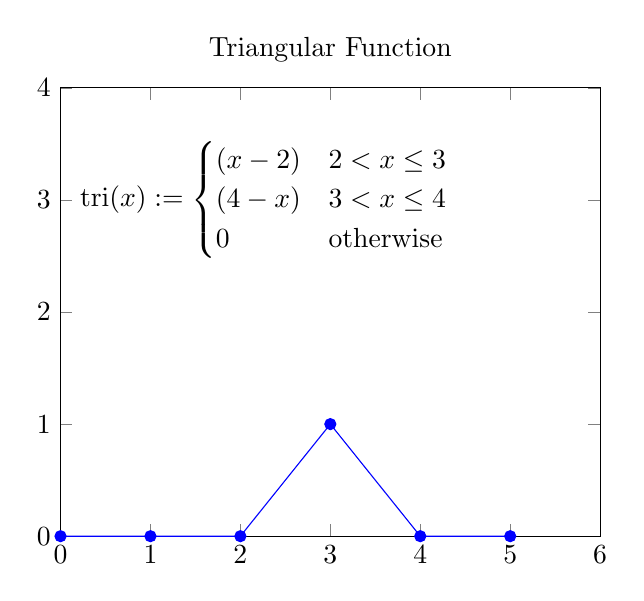
\begin{tikzpicture}
\tikzset{
  every left delimiter/.style={xshift=1ex},
  every label/.style={}
}
\begin{axis}[xmin=0,
             xmax=6,
             ymin=0,
             ymax=4,
             title={Triangular Function}]
  \addplot+[sharp plot, mark=*, mark options={draw=blue, fill=blue}] coordinates
    {(0,0) (1,0) (2,0) (3,1) (4,0) (5,0)};
  \node[label=right:{\parbox[l]{5.0cm}{$\textrm{tri}(x) := \begin{cases} (x-2) & 2 < x \leq 3 \\ (4-x) & 3 < x \leq 4 \\ 0 & \textrm{otherwise}\end{cases}$}}] at (axis description cs:0,0.75) {};
\end{axis}
\end{tikzpicture}


\end{document}
